\documentclass[12pt]{iopart}
\bibliographystyle{unsrt}
\usepackage{cite}
\usepackage[colorlinks, citecolor = blue, urlcolor = blue]{hyperref}
\usepackage{lineno}
\usepackage{longtable}
\usepackage{threeparttable}
\usepackage{threeparttablex}
\usepackage{enumitem}
\usepackage{lscape}
\usepackage{xcolor}
\usepackage{graphicx}
\usepackage[utf8]{inputenc}
\usepackage[T1]{fontenc}
\usepackage{pdfpages}
\usepackage{siunitx}




\begin{document}

\title[Draft - May 2023]{Validation of the code TDCRPy against the code TDCR17 and I2calc}
\author{Romain Coulon}
\address{Bureau International des Poids et Mesures, Pavillon de Breteuil, F-92312 S\`{e}vres Cedex, France.}


\section{Introduction}

The code TDCR17 was developed in Fortran by Philippe Cassette at the LNE-LNHB to calculate the efficiency of a TDCR system. It was used by the LNE-LNHB and other laboratories in key comparisons such as in the CCRI(II)-K2.H-3(2018). I2calc was developed in Python by the BIPM for the same purpose. Both TDCR17 and I2calc realize the numerical summation over a unique energy spectrum. They cannot address complex decay schemes or mixture of radionuclides in solution.\\ 

The BIPM developed the python code TDCRPy to estimating detection efficiency of TDCR measurement. It is a Monte-Carlo TDCR model allowing to calculate efficiency for complex decay scheme or radionuclide mixtures. The aim of this study is to test the BIPM code against the TDCR17 code for pure beta radionuclides planned to be in the scope of the ESIR.\\

\tableofcontents

\pagebreak
\section{Measurement data and results}
\subsection{$^{14}$C}

\begingroup
\footnotesize
\begin{longtable}[l]{| p{.08\textwidth} | p{.08\textwidth} |p{.15\textwidth} |p{.15\textwidth} |p{.15\textwidth} |p{.10\textwidth} |p{.10\textwidth} |} 
\caption{Measurement data and results - $kB = 0.008$ cm $\cdot$ MeV$^{-1}$}
\label{Table1} \\ 
\hline
\textbf{Source} & \textbf{$TDCR$} & \textbf{$\epsilon_{D}$ TDCR17} & \textbf{$\epsilon_{D}$ I2calc} & \textbf{$\epsilon_{D}$ TDCRPy} & err(TD)& err(I2) \\
\endfirsthead
\multicolumn{7}{c}{... Continuation of Table 1.}\\ 
\hline
 \textbf{Source} & \textbf{$TDCR$} & \textbf{$\epsilon_{D}$ TDCR17} & \textbf{$\epsilon_{D}$ I2calc} & \textbf{$\epsilon_{D}$ TDCRPy} & err(TD)& err(I2) \\   \hline 
\endhead
\hline
 1 & 0.9   &   85.37 \% & 91.15 \% & 91.17 \% &  +5.72 \%  & +0.02 \%\\
 2 & 0.8   &   72.88 \% & 83.66 \% & 83.74 \% &  +10.76 \% & +0.08 \%\\
 3 & 0.7   &   61.22 \% & 75.99 \% & 76.15 \% &  +15.09 \% & +0.16 \%\\
 4 & 0.6   &   50.09 \% & 67.68 \% & 67.93 \% &  +17.75 \% & +0.25 \%\\
 5 & 0.5   &   39.35 \% & 58.37 \% & 58.47 \% &  +19.48 \% & +0.10 \%\\
 6 & 0.4   &   29.00 \% & 47.70 \% & 47.77 \% &  +19.17 \% & +0.07 \%\\
 7 & 0.3   &   19.19 \% & 35.42 \% & 35.81 \% &  +16.71 \% & +0.39 \%\\
\hline
\end{longtable} 
\endgroup

\begingroup
\footnotesize
\begin{longtable}[l]{| p{.08\textwidth} | p{.08\textwidth} |p{.15\textwidth} | p{.15\textwidth} |p{.15\textwidth} |p{.10\textwidth} |p{.10\textwidth} |} 
\caption{Measurement data and results - $kB = 0.01$ cm $\cdot$ MeV$^{-1}$}
\label{Table1} \\ 
\hline
\textbf{Source} & \textbf{$TDCR$} & \textbf{$\epsilon_{D}$ TDCR17} & \textbf{$\epsilon_{D}$ I2calc} & \textbf{$\epsilon_{D}$ TDCRPy} & err(TD)& err(I2) \\ 
\endfirsthead
\multicolumn{7}{c}{... Continuation of Table 1.}\\ 
\hline
 \textbf{Source} & \textbf{$TDCR$} & \textbf{$\epsilon_{D}$ TDCR17} & \textbf{$\epsilon_{D}$ I2calc} & \textbf{$\epsilon_{D}$ TDCRPy} & err(TD)& err(I2) \\   \hline 
\endhead
\hline
 1 &  0.9  & 85.17 \% &  90.93 \% & 90.98 \% &  +5.95 \%  & +0.05 \% \\
 2 &  0.8  & 72.60 \% &  83.33 \% & 83.44 \% &  +10.78 \% & +0.11 \% \\
 3 &  0.7  & 60.92 \% &  75.60 \% & 75.77 \% &  +14.96 \% & +0.17 \% \\
 4 &  0.6  & 49.80 \% &  67.27 \% & 67.51 \% &  +17.72 \% & +0.24 \% \\
 5 &  0.5  & 39.09 \% &  57.97 \% & 58.03 \% &  +19.22 \% & +0.06 \% \\
 6 &  0.4  & 28.79 \% &  47.33 \% & 47.42 \% &  +18.96 \% & +0.09 \% \\
 7 &  0.3  & 19.03 \% &  35.12 \% & 35.06 \% &  +16.40 \% & -0.06 \% \\
\hline
\end{longtable} 
\endgroup

\begingroup
\footnotesize
\begin{longtable}[l]{| p{.08\textwidth} | p{.08\textwidth} |p{.15\textwidth} |p{.15\textwidth} |p{.15\textwidth} |p{.10\textwidth} |p{.10\textwidth} |} 
\caption{Measurement data and results - $kB = 0.012$ cm $\cdot$ MeV$^{-1}$}
\label{Table1} \\ 
\hline
\textbf{Source} & \textbf{$TDCR$} & \textbf{$\epsilon_{D}$ TDCR17} & \textbf{$\epsilon_{D}$ I2calc} & \textbf{$\epsilon_{D}$ TDCRPy} & err(TD)& err(I2) \\ 
\endfirsthead
\multicolumn{7}{c}{... Continuation of Table 1.}\\ 
\hline
 \textbf{Source} & \textbf{$TDCR$} & \textbf{$\epsilon_{D}$ TDCR17} & \textbf{$\epsilon_{D}$ I2calc} & \textbf{$\epsilon_{D}$ TDCRPy} & err(TD)& err(I2) \\   \hline 
\endhead
\hline
 1 & 0.9   &  84.98 \% & 90.74 \% & 90.94 \% & +5.82 \%  & +0.20 \% \\
 2 & 0.8   &  72.35 \% & 83.04 \% & 83.10 \% & +10.85 \% & +0.06 \% \\
 3 & 0.7   &  60.65 \% & 75.25 \% & 75.33 \% & +14.88 \% & +0.08 \% \\
 4 & 0.6   &  49.53 \% & 66.90 \% & 67.07 \% & +17.84 \% & +0.17 \% \\
 5 & 0.5   &  38.85 \% & 57.60 \% & 58.06 \% & +18.03 \% & +0.46 \% \\
 6 & 0.4   &  28.60 \% & 47.00 \% & 47.22 \% & +18.75 \% & +0.22 \% \\
 7 & 0.3   &  18.89 \% & 34.85 \% & 35.05 \% & +15.78 \% & +0.20 \% \\
\hline
\end{longtable} 
\endgroup

At $TDCR = 0.8$, $\Delta \epsilon_D = |83.74 - 83.10| = 0.64 \%$ for $kB = [0.008, 0.012]$ cm/MeV. The difference with TDCR17 is largely higher $\approx 11 \%$. There is a problem probably due to the beta spectrum evaluation. Indeed, the difference with I2calc, using betaShape, is lower :  $\approx 0.10 \%$. 


\pagebreak
\subsection{$^{63}$Ni}

\begingroup
\footnotesize
\begin{longtable}[l]{| p{.08\textwidth} | p{.08\textwidth} |p{.15\textwidth} |p{.15\textwidth} |p{.15\textwidth} |p{.10\textwidth} |p{.10\textwidth} |} 
\caption{Measurement data and results - $kB = 0.008$ cm $\cdot$ MeV$^{-1}$}
\label{Table1} \\ 
\hline
\textbf{Source} & \textbf{$TDCR$} & \textbf{$\epsilon_{D}$ TDCR17} & \textbf{$\epsilon_{D}$ I2calc} & \textbf{$\epsilon_{D}$ TDCRPy} & err(TD)& err(I2) \\
\endfirsthead
\multicolumn{7}{c}{... Continuation of Table 1.}\\ 
\hline
 \textbf{Source} & \textbf{$TDCR$} & \textbf{$\epsilon_{D}$ TDCR17} & \textbf{$\epsilon_{D}$ I2calc} & \textbf{$\epsilon_{D}$ TDCRPy} & err(TD)& err(I2) \\   \hline 
\endhead
\hline
 1 & 0.9   &   89.34 \% &  & 89.38 \% &  +0.04 \% & \\
 2 & 0.8   &   79.86 \% &  & 79.79 \% &  -0.07 \% & \\
 3 & 0.7   &   70.80 \% &  & 70.70 \% &  -0.10 \% & \\
 4 & 0.6   &   61.68 \% &  & 61.28 \% &  -0.40 \% & \\
 5 & 0.5   &   52.12 \% &  & 51.42 \% &  -0.70 \% & \\
 6 & 0.4   &   41.78 \% &  & 41.01 \% &  -0.77 \% & \\
 7 & 0.3   &   30.46 \% &  & 29.88 \% &  -0.58 \% & \\
\hline
\end{longtable} 
\endgroup


\begingroup
\footnotesize
\begin{longtable}[l]{| p{.08\textwidth} | p{.08\textwidth} |p{.15\textwidth} | p{.15\textwidth} |p{.15\textwidth} |p{.10\textwidth} |p{.10\textwidth} |} 
\caption{Measurement data and results - $kB = 0.01$ cm $\cdot$ MeV$^{-1}$}
\label{Table1} \\ 
\hline
\textbf{Source} & \textbf{$TDCR$} & \textbf{$\epsilon_{D}$ TDCR17} & \textbf{$\epsilon_{D}$ I2calc} & \textbf{$\epsilon_{D}$ TDCRPy} & err(TD)& err(I2) \\ 
\endfirsthead
\multicolumn{7}{c}{... Continuation of Table 1.}\\ 
\hline
 \textbf{Source} & \textbf{$TDCR$} & \textbf{$\epsilon_{D}$ TDCR17} & \textbf{$\epsilon_{D}$ I2calc} & \textbf{$\epsilon_{D}$ TDCRPy} & err(TD)& err(I2) \\   \hline 
\endhead
\hline
 1 &  0.9  &  89.03 \% &  & 88.98 \% & -0.05 \% & \\
 2 &  0.8  &  79.35 \% &  & 79.54 \% & +0.20 \% & \\
 3 &  0.7  &  70.19 \% &  & 70.27 \% & +0.08 \% & \\
 4 &  0.6  &  61.04 \% &  & 60.69 \% & -0.35 \% & \\
 5 &  0.5  &  51.49 \% &  & 50.78 \% & -0.71 \% & \\
 6 &  0.4  &  41.22 \% &  & 40.24 \% & -0.98 \% & \\
 7 &  0.3  &  30.02 \% &  & 29.12 \% & -0.90 \% & \\
\hline
\end{longtable} 
\endgroup

\begingroup
\footnotesize
\begin{longtable}[l]{| p{.08\textwidth} | p{.08\textwidth} |p{.15\textwidth} |p{.15\textwidth} |p{.15\textwidth} |p{.10\textwidth} |p{.10\textwidth} |} 
\caption{Measurement data and results - $kB = 0.012$ cm $\cdot$ MeV$^{-1}$}
\label{Table1} \\ 
\hline
\textbf{Source} & \textbf{$TDCR$} & \textbf{$\epsilon_{D}$ TDCR17} & \textbf{$\epsilon_{D}$ I2calc} & \textbf{$\epsilon_{D}$ TDCRPy} & err(TD)& err(I2) \\ 
\endfirsthead
\multicolumn{7}{c}{... Continuation of Table 1.}\\ 
\hline
 \textbf{Source} & \textbf{$TDCR$} & \textbf{$\epsilon_{D}$ TDCR17} & \textbf{$\epsilon_{D}$ I2calc} & \textbf{$\epsilon_{D}$ TDCRPy} & err(TD)& err(I2) \\   \hline 
\endhead
\hline
 1 & 0.9   &   88.75 \% &  & 88.81 \% & +0.06 \% & \\
 2 & 0.8   &   78.91 \% &  & 79.07 \% & +0.16 \% & \\
 3 & 0.7   &   69.66 \% &  & 69.76 \% & +0.10 \% & \\
 4 & 0.6   &   60.47 \% &  & 60.27 \% & -0.20 \% & \\
 5 & 0.5   &   50.94 \% &  & 50.30 \% & -0.64 \% & \\
 6 & 0.4   &   40.73 \% &  & 39.81 \% & -0.92 \% & \\
 7 & 0.3   &   29.63 \% &  & 28.78 \% & -0.85 \% & \\
\hline
\end{longtable} 
\endgroup

At $TDCR = 0.8$, $\Delta \epsilon_D = |79.07 - 79.79| = 0.72 \%$ for $kB = [0.008, 0.012]$ cm/MeV. The difference between software is lower $\approx 0.2 \%$. 

\pagebreak
\subsection{$^{3}$H}

\begingroup
\footnotesize
\begin{longtable}[l]{| p{.08\textwidth} | p{.08\textwidth} |p{.15\textwidth} |p{.15\textwidth} |p{.15\textwidth} |p{.10\textwidth} |p{.10\textwidth} |} 
\caption{Measurement data and results - $kB = 0.008$ cm $\cdot$ MeV$^{-1}$}
\label{Table1} \\ 
\hline
\textbf{Source} & \textbf{$TDCR$} & \textbf{$\epsilon_{D}$ TDCR17} & \textbf{$\epsilon_{D}$ I2calc} & \textbf{$\epsilon_{D}$ TDCRPy} & err(TD)& err(I2) \\
\endfirsthead
\multicolumn{7}{c}{... Continuation of Table 1.}\\ 
\hline
 \textbf{Source} & \textbf{$TDCR$} & \textbf{$\epsilon_{D}$ TDCR17} & \textbf{$\epsilon_{D}$ I2calc} & \textbf{$\epsilon_{D}$ TDCRPy} & err(TD)& err(I2) \\   \hline 
\endhead
\hline
 1 & 0.9   &   90.42 \% &  & 90.73 \% &  +0.31 \% & \\
 2 & 0.8   &   81.92 \% &  & 82.20 \% &  +0.28 \% & \\
 3 & 0.7   &   73.51 \% &  & 73.66 \% &  +0.15 \% & \\
 4 & 0.6   &   64.75 \% &  & 64.60 \% &  -0.10 \% & \\
 5 & 0.5   &   55.25 \% &  & 54.79 \% &  -0.46 \% & \\
 6 & 0.4   &   44.70 \% &  & 44.14 \% &  -0.56 \% & \\
 7 & 0.3   &   32.87 \% &  & 32.51 \% &  -0.36 \% & \\
\hline
\end{longtable} 
\endgroup

\begingroup
\footnotesize
\begin{longtable}[l]{| p{.08\textwidth} | p{.08\textwidth} |p{.15\textwidth} | p{.15\textwidth} |p{.15\textwidth} |p{.10\textwidth} |p{.10\textwidth} |} 
\caption{Measurement data and results - $kB = 0.01$ cm $\cdot$ MeV$^{-1}$}
\label{Table1} \\ 
\hline
\textbf{Source} & \textbf{$TDCR$} & \textbf{$\epsilon_{D}$ TDCR17} & \textbf{$\epsilon_{D}$ I2calc} & \textbf{$\epsilon_{D}$ TDCRPy} & err(TD)& err(I2) \\ 
\endfirsthead
\multicolumn{7}{c}{... Continuation of Table 1.}\\ 
\hline
 \textbf{Source} & \textbf{$TDCR$} & \textbf{$\epsilon_{D}$ TDCR17} & \textbf{$\epsilon_{D}$ I2calc} & \textbf{$\epsilon_{D}$ TDCRPy} & err(TD)& err(I2) \\   \hline 
\endhead
\hline
 1 &  0.9  &  90.17 \% &  & 90.58 \% &  +0.41 \% & \\
 2 &  0.8  &  81.44 \% &  & 81.72 \% &  +0.28 \% & \\
 3 &  0.7  &  72.88 \% &  & 73.07 \% &  +0.19 \% & \\
 4 &  0.6  &  64.03 \% &  & 63.99 \% &  -0.04 \% & \\
 5 &  0.5  &  54.51 \% &  & 54.37 \% &  -0.14 \% & \\
 6 &  0.4  &  44.00 \% &  & 43.74 \% &  -0.26 \% & \\
 7 &  0.3  &  32.29 \% &  & 31.96 \% &  -0.33 \% & \\
\hline
\end{longtable} 
\endgroup

\begingroup
\footnotesize
\begin{longtable}[l]{| p{.08\textwidth} | p{.08\textwidth} |p{.15\textwidth} |p{.15\textwidth} |p{.15\textwidth} |p{.10\textwidth} |p{.10\textwidth} |} 
\caption{Measurement data and results - $kB = 0.012$ cm $\cdot$ MeV$^{-1}$}
\label{Table1} \\ 
\hline
\textbf{Source} & \textbf{$TDCR$} & \textbf{$\epsilon_{D}$ TDCR17} & \textbf{$\epsilon_{D}$ I2calc} & \textbf{$\epsilon_{D}$ TDCRPy} & err(TD)& err(I2) \\ 
\endfirsthead
\multicolumn{7}{c}{... Continuation of Table 1.}\\ 
\hline
 \textbf{Source} & \textbf{$TDCR$} & \textbf{$\epsilon_{D}$ TDCR17} & \textbf{$\epsilon_{D}$ I2calc} & \textbf{$\epsilon_{D}$ TDCRPy} & err(TD)& err(I2) \\   \hline 
\endhead
\hline
 1 & 0.9   &   89.96 \% &  & 90.43 \% & +0.47 \% & \\
 2 & 0.8   &   81.04 \% &  & 81.34 \% & +0.30 \% & \\
 3 & 0.7   &   72.34 \% &  & 72.55 \% & +0.21 \% & \\
 4 & 0.6   &   63.42 \% &  & 63.61 \% & +0.19 \% & \\
 5 & 0.5   &   53.88 \% &  & 53.69 \% & -0.19 \% & \\
 6 & 0.4   &   43.41 \% &  & 42.77 \% & -0.64 \% & \\
 7 & 0.3   &   31.80 \% &  & 31.12 \% & -0.68 \% & \\
\hline
\end{longtable} 
\endgroup

At $TDCR = 0.7$, $\Delta \epsilon_D = |72.55 - 73.66| = 1.11 \%$ for $kB = [0.008, 0.012]$ cm/MeV. The difference between software is lower $\approx 0.2 \%$ . 

\pagebreak
\subsection{$^{35}$S}

\begingroup
\footnotesize
\begin{longtable}[l]{| p{.08\textwidth} | p{.08\textwidth} |p{.15\textwidth} |p{.15\textwidth} |p{.15\textwidth} |p{.10\textwidth} |p{.10\textwidth} |} 
\caption{Measurement data and results - $kB = 0.008$ cm $\cdot$ MeV$^{-1}$}
\label{Table1} \\ 
\hline
\textbf{Source} & \textbf{$TDCR$} & \textbf{$\epsilon_{D}$ TDCR17} & \textbf{$\epsilon_{D}$ I2calc} & \textbf{$\epsilon_{D}$ TDCRPy} & err(TD)& err(I2) \\
\endfirsthead
\multicolumn{7}{c}{... Continuation of Table 1.}\\ 
\hline
 \textbf{Source} & \textbf{$TDCR$} & \textbf{$\epsilon_{D}$ TDCR17} & \textbf{$\epsilon_{D}$ I2calc} & \textbf{$\epsilon_{D}$ TDCRPy} & err(TD)& err(I2) \\   \hline 
\endhead
\hline
 1 & 0.9   &   90.34 \% &  &  89.85 \% &  -0.49 \% & \\
 2 & 0.8   &   82.01 \% &  &  81.64 \% &  -0.37 \% & \\
 3 & 0.7   &   73.88 \% &  &  73.48 \% &  -0.40 \% & \\
 4 & 0.6   &   65.37 \% &  &  64.78 \% &  -0.59 \% & \\
 5 & 0.5   &   56.07 \% &  &  55.07 \% &  -1.00 \% & \\
 6 & 0.4   &   45.61 \% &  &  44.23 \% &  -1.38 \% & \\
 7 & 0.3   &   33.73 \% &  &  32.66 \% &  -1.07 \% & \\
\hline
\end{longtable} 
\endgroup


\begingroup
\footnotesize
\begin{longtable}[l]{| p{.08\textwidth} | p{.08\textwidth} |p{.15\textwidth} | p{.15\textwidth} |p{.15\textwidth} |p{.10\textwidth} |p{.10\textwidth} |} 
\caption{Measurement data and results - $kB = 0.01$ cm $\cdot$ MeV$^{-1}$}
\label{Table1} \\ 
\hline
\textbf{Source} & \textbf{$TDCR$} & \textbf{$\epsilon_{D}$ TDCR17} & \textbf{$\epsilon_{D}$ I2calc} & \textbf{$\epsilon_{D}$ TDCRPy} & err(TD)& err(I2) \\ 
\endfirsthead
\multicolumn{7}{c}{... Continuation of Table 1.}\\ 
\hline
 \textbf{Source} & \textbf{$TDCR$} & \textbf{$\epsilon_{D}$ TDCR17} & \textbf{$\epsilon_{D}$ I2calc} & \textbf{$\epsilon_{D}$ TDCRPy} & err(TD)& err(I2) \\   \hline 
\endhead
\hline
 1 &  0.9  &  90.08 \% &  & 89.74 \% &  -0.34 \% & \\
 2 &  0.8  &  81.65 \% &  & 81.28 \% &  -0.37 \% & \\
 3 &  0.7  &  73.47 \% &  & 73.07 \% &  -0.40 \% & \\
 4 &  0.6  &  64.95 \% &  & 64.36 \% &  -0.59 \% & \\
 5 &  0.5  &  55.67 \% &  & 54.78 \% &  -0.89 \% & \\
 6 &  0.4  &  45.25 \% &  & 44.19 \% &  -1.06 \% & \\
 7 &  0.3  &  33.44 \% &  & 32.84 \% &  -0.60 \% & \\
\hline
\end{longtable} 
\endgroup

\begingroup
\footnotesize
\begin{longtable}[l]{| p{.08\textwidth} | p{.08\textwidth} |p{.15\textwidth} |p{.15\textwidth} |p{.15\textwidth} |p{.10\textwidth} |p{.10\textwidth} |} 
\caption{Measurement data and results - $kB = 0.012$ cm $\cdot$ MeV$^{-1}$}
\label{Table1} \\ 
\hline
\textbf{Source} & \textbf{$TDCR$} & \textbf{$\epsilon_{D}$ TDCR17} & \textbf{$\epsilon_{D}$ I2calc} & \textbf{$\epsilon_{D}$ TDCRPy} & err(TD)& err(I2) \\ 
\endfirsthead
\multicolumn{7}{c}{... Continuation of Table 1.}\\ 
\hline
 \textbf{Source} & \textbf{$TDCR$} & \textbf{$\epsilon_{D}$ TDCR17} & \textbf{$\epsilon_{D}$ I2calc} & \textbf{$\epsilon_{D}$ TDCRPy} & err(TD)& err(I2) \\   \hline 
\endhead
\hline
 1 & 0.9   &   89.86 \% &  & 89.40 \% &  -0.46 \% & \\
 2 & 0.8   &   81.33 \% &  & 80.87 \% &  -0.46 \% & \\
 3 & 0.7   &   73.10 \% &  & 72.42 \% &  -0.68 \% & \\
 4 & 0.6   &   64.57 \% &  & 63.84 \% &  -0.73 \% & \\
 5 & 0.5   &   55.30 \% &  & 54.27 \% &  -1.03 \% & \\
 6 & 0.4   &   44.92 \% &  & 43.99 \% &  -0.93 \% & \\
 7 & 0.3   &   33.18 \% &  & 32.43 \% &  -0.75 \% & \\
\hline
\end{longtable} 
\endgroup

At $TDCR = 0.8$, $\Delta \epsilon_D = |80.87 - 81.64| = 0.77 \%$ for $kB = [0.008, 0.012]$ cm/MeV. The difference between software is lower $\approx 0.4 \%$ . 


\pagebreak
\subsection{$^{U}$X}

\begingroup
\footnotesize
\begin{longtable}[l]{| p{.08\textwidth} | p{.08\textwidth} |p{.15\textwidth} |p{.15\textwidth} |p{.15\textwidth} |p{.10\textwidth} |p{.10\textwidth} |} 
\caption{Measurement data and results - $kB = 0.008$ cm $\cdot$ MeV$^{-1}$}
\label{Table1} \\ 
\hline
\textbf{Source} & \textbf{$TDCR$} & \textbf{$\epsilon_{D}$ TDCR17} & \textbf{$\epsilon_{D}$ I2calc} & \textbf{$\epsilon_{D}$ TDCRPy} & err(TD)& err(I2) \\
\endfirsthead
\multicolumn{7}{c}{... Continuation of Table 1.}\\ 
\hline
 \textbf{Source} & \textbf{$TDCR$} & \textbf{$\epsilon_{D}$ TDCR17} & \textbf{$\epsilon_{D}$ I2calc} & \textbf{$\epsilon_{D}$ TDCRPy} & err(TD)& err(I2) \\   \hline 
\endhead
\hline
 1 & 0.9   &    \% & \% &  \% &   \% &   \%\\
 2 & 0.8   &    \% & \% &  \% &   \% &   \%\\
 3 & 0.7   &    \% & \% &  \% &   \% &   \%\\
 4 & 0.6   &    \% & \% &  \% &   \% &   \%\\
 5 & 0.5   &    \% & \% &  \% &   \% &   \%\\
 6 & 0.4   &    \% & \% &  \% &   \% &   \%\\
 7 & 0.3   &    \% & \% &  \% &   \% &   \%\\
\hline
\end{longtable} 
\endgroup


\begingroup
\footnotesize
\begin{longtable}[l]{| p{.08\textwidth} | p{.08\textwidth} |p{.15\textwidth} | p{.15\textwidth} |p{.15\textwidth} |p{.10\textwidth} |p{.10\textwidth} |} 
\caption{Measurement data and results - $kB = 0.01$ cm $\cdot$ MeV$^{-1}$}
\label{Table1} \\ 
\hline
\textbf{Source} & \textbf{$TDCR$} & \textbf{$\epsilon_{D}$ TDCR17} & \textbf{$\epsilon_{D}$ I2calc} & \textbf{$\epsilon_{D}$ TDCRPy} & err(TD)& err(I2) \\ 
\endfirsthead
\multicolumn{7}{c}{... Continuation of Table 1.}\\ 
\hline
 \textbf{Source} & \textbf{$TDCR$} & \textbf{$\epsilon_{D}$ TDCR17} & \textbf{$\epsilon_{D}$ I2calc} & \textbf{$\epsilon_{D}$ TDCRPy} & err(TD)& err(I2) \\   \hline 
\endhead
\hline
 1 & 0.9   &    \% & \% &  \% &   \% &   \%\\
 2 & 0.8   &    \% & \% &  \% &   \% &   \%\\
 3 & 0.7   &    \% & \% &  \% &   \% &   \%\\
 4 & 0.6   &    \% & \% &  \% &   \% &   \%\\
 5 & 0.5   &    \% & \% &  \% &   \% &   \%\\
 6 & 0.4   &    \% & \% &  \% &   \% &   \%\\
 7 & 0.3   &    \% & \% &  \% &   \% &   \%\\
\hline
\end{longtable} 
\endgroup

\begingroup
\footnotesize
\begin{longtable}[l]{| p{.08\textwidth} | p{.08\textwidth} |p{.15\textwidth} |p{.15\textwidth} |p{.15\textwidth} |p{.10\textwidth} |p{.10\textwidth} |} 
\caption{Measurement data and results - $kB = 0.012$ cm $\cdot$ MeV$^{-1}$}
\label{Table1} \\ 
\hline
\textbf{Source} & \textbf{$TDCR$} & \textbf{$\epsilon_{D}$ TDCR17} & \textbf{$\epsilon_{D}$ I2calc} & \textbf{$\epsilon_{D}$ TDCRPy} & err(TD)& err(I2) \\ 
\endfirsthead
\multicolumn{7}{c}{... Continuation of Table 1.}\\ 
\hline
 \textbf{Source} & \textbf{$TDCR$} & \textbf{$\epsilon_{D}$ TDCR17} & \textbf{$\epsilon_{D}$ I2calc} & \textbf{$\epsilon_{D}$ TDCRPy} & err(TD)& err(I2) \\   \hline 
\endhead
\hline
 1 & 0.9   &    \% & \% &  \% &   \% &   \%\\
 2 & 0.8   &    \% & \% &  \% &   \% &   \%\\
 3 & 0.7   &    \% & \% &  \% &   \% &   \%\\
 4 & 0.6   &    \% & \% &  \% &   \% &   \%\\
 5 & 0.5   &    \% & \% &  \% &   \% &   \%\\
 6 & 0.4   &    \% & \% &  \% &   \% &   \%\\
 7 & 0.3   &    \% & \% &  \% &   \% &   \%\\
\hline
\end{longtable} 
\endgroup

\pagebreak
\section{Spectra}

\begin{figure}[h!]
\centering
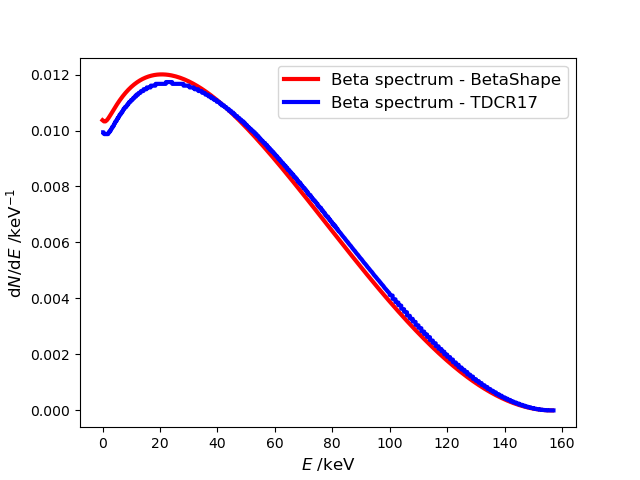
\includegraphics[scale=0.4]{../decayData/spectra/BetaSpectrum_C-14.png}
\caption{$\beta$ spectra of $^{14}$C from BetaShape (used in TDCRPy) and TDCR17}
\label{fig:C-14}
\end{figure}

\begin{figure}[h!]
\centering
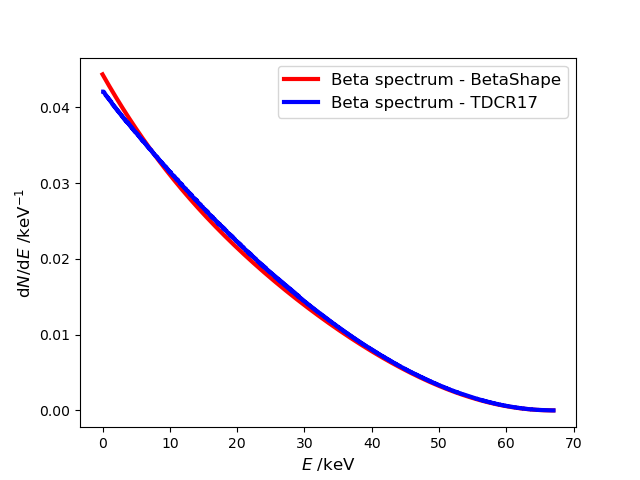
\includegraphics[scale=0.4]{../decayData/spectra/BetaSpectrum_Ni-63.png}
\caption{$\beta$ spectra of $^{63}$Ni from BetaShape (used in TDCRPy) and TDCR17}
\label{fig:Ni-63}
\end{figure}

\begin{figure}[h!]
\centering
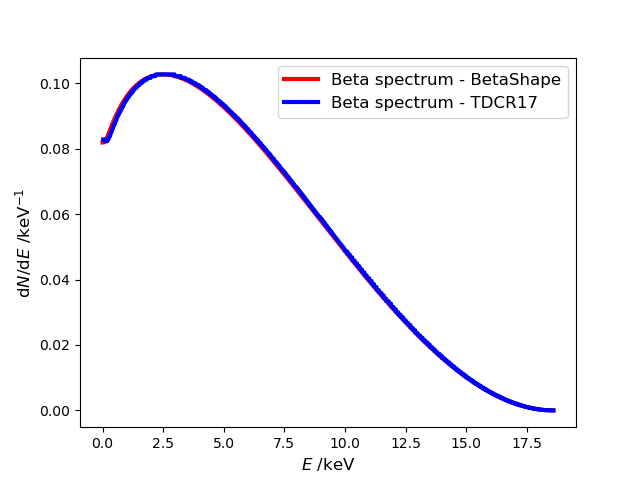
\includegraphics[scale=0.4]{../decayData/spectra/BetaSpectrum_H-3.png}
\caption{$\beta$ spectra of $^{3}$H from BetaShape (used in TDCRPy) and TDCR17}
\label{fig:H-3}
\end{figure}

\begin{figure}[h!]
\centering
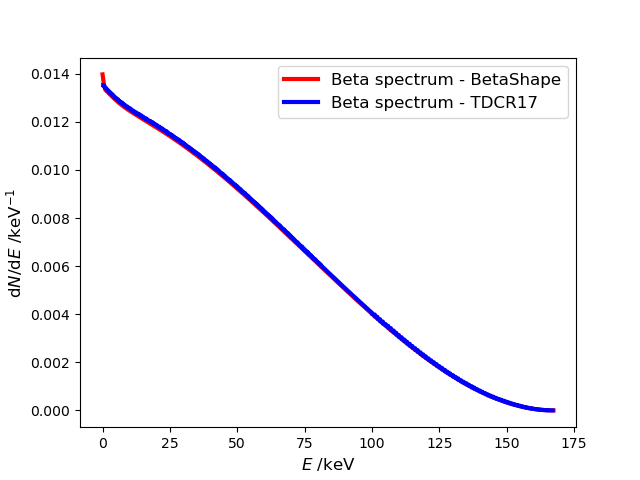
\includegraphics[scale=0.4]{../decayData/spectra/BetaSpectrum_S-35.png}
\caption{$\beta$ spectra of $^{35}$S from BetaShape (used in TDCRPy) and TDCR17}
\label{fig:S-35}
\end{figure}

\end{document}